%%%%%%%%%%%%%%%%%%%%%%%%
%
% $Autor: Hemanth Jadiswami Prabhakaran $
% $Datum: 2025-06-29 19:45:32Z $
% $Pfad: GitHub/BA25-01-Time-Series/report/Contents/en/pmdarima.tex $
% $Version: 1 $
%
% $Project: BA25-Time-Series $
%
%%%%%%%%%%%%%%%%%%%%%%%%


%
% !TeX encoding = utf8
% !TeX root = PythonPackages
%
%%%%%%%%%%%%%%%%%%%%%%%%

\chapter{Pmdarima}
\label{ch:pmdarima}

\section{Introduction}
\label{sec:intro}

Pmdarima represents a revolutionary approach to time series forecasting by bringing R's beloved auto.arima functionality to Python \cite{Pmdarima:2024}. Originally named pyramid-arima (an anagram of 'py' + 'arima'), this statistical library was designed to fill the critical void in Python's time series analysis capabilities. Created by Taylor G. Smith and maintained by a dedicated team of volunteers, pmdarima has become an indispensable tool for data scientists working with temporal data \cite{Smith:2023}. The library provides automatic ARIMA model selection, seasonal modeling capabilities, and a scikit-learn-compatible interface that democratizes advanced time series forecasting for practitioners at all levels.\\

The significance of pmdarima in the time series forecasting landscape cannot be overstated. Traditional ARIMA modeling required extensive domain knowledge to manually select optimal parameters through iterative testing of different combinations. Pmdarima eliminates this complexity by implementing sophisticated statistical tests and optimization algorithms that automatically determine the best model configuration \cite{HyndmanKhandakar:2008}. Modern data science workflows benefit tremendously from pmdarima's ability to seamlessly integrate with existing Python ecosystems while providing state-of-the-art forecasting capabilities. The library's emphasis on automation, combined with its robust handling of seasonal patterns and exogenous variables, has made it a cornerstone package for time series analysis in production environments worldwide.\\

\section{Description}
\label{sec:description}

\subsection{Core Capabilities}
\label{subsec:capabilities}

Pmdarima offers a comprehensive suite of time series forecasting capabilities:

\begin{itemize}
	\item \textbf{Automatic ARIMA Selection}: Automated parameter tuning using statistical tests and information criteria
	\item \textbf{Seasonal Modeling}: Native support for SARIMA and SARIMAX models with automatic seasonality detection
	\item \textbf{Scikit-learn Compatibility}: Familiar fit/predict interface for seamless integration with ML pipelines
	\item \textbf{Statistical Testing}: Built-in stationarity and seasonality tests for robust model validation
	\item \textbf{Preprocessing Pipeline}: Comprehensive transformers including Box-Cox and Fourier transformations
\end{itemize}

\clearpage

\subsection{Python Framework: pmdarima}
\label{subsec:pmdarima}

The \texttt{pmdarima} package wraps statsmodels under the hood while providing an intuitive, sklearn-style interface. It offers powerful automatic model selection through the auto\_arima function:

\begin{lstlisting}[language=MyPython, caption={Pmdarima Core Functions}, label={lst:pmdarima_core}]
	
	import pmdarima as pm
	from pmdarima.model_selection import train_test_split
	import numpy as np
	
	# Load and split data
	y = pm.datasets.load_wineind()
	train, test = train_test_split(y, train_size=150)
	
	# Automatic ARIMA model selection
	model = pm.auto_arima(train, seasonal=True, m=12)
	
	# Make forecasts
	forecasts = model.predict(test.shape[0])
	
\end{lstlisting}

\subsection{Use Cases}
\label{subsec:usecases}

Pmdarima finds applications across diverse time series forecasting domains:

\begin{enumerate}
	\item \textbf{Financial Forecasting}: Stock price prediction, revenue forecasting, and risk modeling
	\item \textbf{Demand Planning}: Inventory management, supply chain optimization, and resource allocation
	\item \textbf{Weather Prediction}: Climate modeling, seasonal pattern analysis, and environmental monitoring
	\item \textbf{Business Analytics}: Sales forecasting, customer behavior analysis, and performance metrics
	\item \textbf{IoT and Sensor Data}: Industrial monitoring, predictive maintenance, and anomaly detection
\end{enumerate}

\subsection{Architecture Overview}
\label{subsec:architecture}

\begin{figure}[H]
	\centering
	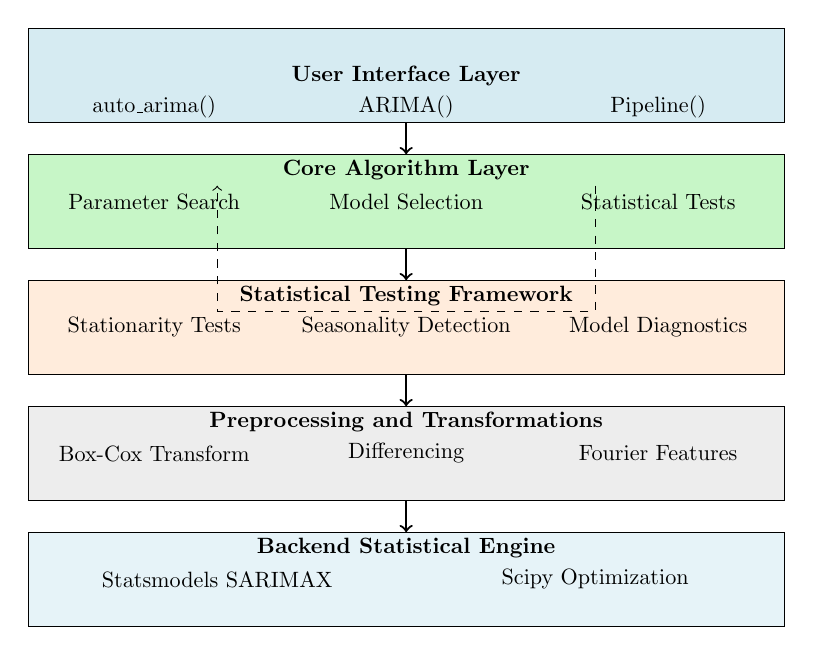
\begin{tikzpicture}[scale=0.8, every node/.style={scale=0.8}]

% Define colors
\definecolor{lightblue}{RGB}{173,216,230}
\definecolor{lightgreen}{RGB}{144,238,144}
\definecolor{lightorange}{RGB}{255,218,185}
\definecolor{lightgray}{RGB}{220,220,220}

% User Interface Layer
\draw[fill=lightblue!50] (0,8) rectangle (12,9.5);
\node at (6,8.75) {\textbf{User Interface Layer}};
\node at (2,8.25) {auto\_arima()};
\node at (6,8.25) {ARIMA()};
\node at (10,8.25) {Pipeline()};

% Core Algorithm Layer
\draw[fill=lightgreen!50] (0,6) rectangle (12,7.5);
\node at (6,7.25) {\textbf{Core Algorithm Layer}};
\node at (2,6.75) {Parameter Search};
\node at (6,6.75) {Model Selection};
\node at (10,6.75) {Statistical Tests};

% Statistical Tests
\draw[fill=lightorange!50] (0,4) rectangle (12,5.5);
\node at (6,5.25) {\textbf{Statistical Testing Framework}};
\node at (2,4.75) {Stationarity Tests};
\node at (6,4.75) {Seasonality Detection};
\node at (10,4.75) {Model Diagnostics};

% Preprocessing Layer
\draw[fill=lightgray!50] (0,2) rectangle (12,3.5);
\node at (6,3.25) {\textbf{Preprocessing and Transformations}};
\node at (2,2.75) {Box-Cox Transform};
\node at (6,2.75) {Differencing};
\node at (10,2.75) {Fourier Features};

% Backend Layer
\draw[fill=lightblue!30] (0,0) rectangle (12,1.5);
\node at (6,1.25) {\textbf{Backend Statistical Engine}};
\node at (3,0.75) {Statsmodels SARIMAX};
\node at (9,0.75) {Scipy Optimization};

% Arrows showing data flow
\draw[->, thick] (6,8) -- (6,7.5);
\draw[->, thick] (6,6) -- (6,5.5);
\draw[->, thick] (6,4) -- (6,3.5);
\draw[->, thick] (6,2) -- (6,1.5);

% Side arrows for feedback loops
\draw[->, dashed] (9,7) -- (9,5) -- (3,5) -- (3,7);

\end{tikzpicture}
	\caption{Pmdarima Library Architecture \cite{Pmdarima:2024}}
	\label{fig:pmdarima_architecture}
\end{figure}

The pmdarima architecture employs a layered approach, as illustrated in Figure \ref{fig:pmdarima_architecture}. The library builds upon statsmodels' robust statistical foundations while providing automated parameter selection through sophisticated search algorithms. This architecture enables both novice and expert users to leverage advanced time series modeling techniques \cite{Smith:2023}.

\clearpage

\section{Installation}
\label{sec:installation}

\subsection{System Requirements}
\label{subsec:system_requirements}

Pmdarima requires Python 3.7 or higher and has the following core dependencies:
\begin{itemize}
	\item NumPy (>= 1.19.3)
	\item Pandas (>= 0.19)
	\item SciPy (>= 1.3.2)
	\item Statsmodels (!= 0.12.0, >= 0.11)
	\item Scikit-learn (>= 0.22)
	\item Joblib (>= 0.11)
\end{itemize}

\subsection{Python Package Installation}
\label{subsec:python_install}

Install pmdarima using pip or conda:

\begin{lstlisting}[style=bashstyle, caption={Pmdarima Installation}]
	# Standard installation
	pip install pmdarima
	
	# With additional dependencies for enhanced functionality
	pip install pmdarima[complete]
	
	# Conda installation
	conda config --add channels conda-forge
	conda config --set channel_priority strict
	conda install pmdarima
\end{lstlisting}

\subsection{Building from Source}
\label{subsec:source_install}

For development or latest features, build from source:

\begin{lstlisting}[style=bashstyle, caption={Source Installation}]
	# Clone repository
	git clone https://github.com/alkaline-ml/pmdarima.git
	cd pmdarima
	
	# Install build dependencies
	pip install cython>=0.29
	
	# Build and install
	python setup.py install
\end{lstlisting}

\subsection{Verification}
\label{subsec:verification}

Verify the installation:

\begin{lstlisting}[language=MyPython, caption={Installation Verification}]
	import pmdarima as pm
	print(pm.__version__)
	
	# Test with sample data
	y = pm.datasets.load_wineind()
	model = pm.auto_arima(y, seasonal=True, m=12, 
	                      suppress_warnings=True)
	print("Installation successful!")
\end{lstlisting}

\section{Example -- Basic Time Series Forecasting}
\label{sec:basic_example}

The following example demonstrates automatic ARIMA model selection and forecasting using pmdarima's core functionality. The complete implementation is available in \texttt{BasicForecasting.py}.

\lstinputlisting[language=MyPython, caption={Basic Time Series Forecasting}, label={lst:basicforecasting},firstline=1,lastline=50]{../Code/pmdarima/BasicForecasting.py}

\noindent\textit{[The remaining code is omitted for brevity. The complete script can be found at \texttt{../Code/pmdarima/BasicForecasting.py}.]}

This basic example illustrates pmdarima's fundamental workflow: automatic model selection, fitting, and forecasting. The auto\_arima function automatically determines optimal parameters through statistical testing and information criteria optimization.

\section{Example -- Seasonal ARIMA with Exogenous Variables}
\label{sec:seasonal_example}

Advanced pmdarima applications leverage seasonal patterns and external variables for enhanced forecasting accuracy. The SARIMAX framework enables incorporation of exogenous regressors alongside seasonal modeling.

\clearpage

\begin{figure}[htbp]
	\centering
    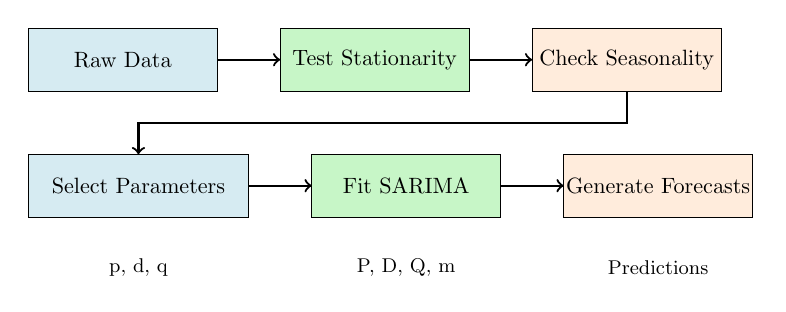
\begin{tikzpicture}[scale=0.8, every node/.style={scale=0.8}]
	
	% Define colors
	\definecolor{lightblue}{RGB}{173,216,230}
	\definecolor{lightgreen}{RGB}{144,238,144}
	\definecolor{lightorange}{RGB}{255,218,185}
	
	% Simple linear flow with wider boxes
	\draw[fill=lightblue!50] (0,6) rectangle (3,7);
	\node at (1.5,6.5) {Raw Data};
	
	\draw[fill=lightgreen!50] (4,6) rectangle (7,7);
	\node at (5.5,6.5) {Test Stationarity};
	
	\draw[fill=lightorange!50] (8,6) rectangle (11,7);
	\node at (9.5,6.5) {Check Seasonality};
	
	\draw[fill=lightblue!50] (0,4) rectangle (3.5,5);
	\node at (1.75,4.5) {Select Parameters};
	
	\draw[fill=lightgreen!50] (4.5,4) rectangle (7.5,5);
	\node at (6,4.5) {Fit SARIMA};
	
	\draw[fill=lightorange!50] (8.5,4) rectangle (11.5,5);
	\node at (10,4.5) {Generate Forecasts};
	
	% Correct sequential arrows
	\draw[->, thick] (3,6.5) -- (4,6.5);
	\draw[->, thick] (7,6.5) -- (8,6.5);
	\draw[->, thick] (9.5,6) -- (9.5,5.5) -- (1.75,5.5) -- (1.75,5);
	\draw[->, thick] (3.5,4.5) -- (4.5,4.5);
	\draw[->, thick] (7.5,4.5) -- (8.5,4.5);
	
	% Labels
	\node at (1.75,3.2) {\small p, d, q};
	\node at (6,3.2) {\small P, D, Q, m};
	\node at (10,3.2) {\small Predictions};
	
\end{tikzpicture}
	\caption{Seasonal ARIMA Modeling Workflow}
	\label{fig:seasonal_flow}
\end{figure}

The seasonal modeling workflow illustrated in Figure \ref{fig:seasonal_flow} shows the comprehensive process from data preprocessing through model validation and forecasting.

\lstinputlisting[language=MyPython, caption={Seasonal ARIMA with Exogenous Variables}, label={lst:seasonalarima},firstline=1,lastline=50]{../Code/pmdarima/SeasonalARIMA.py}
\noindent\textit{The remaining code is omitted for brevity. The complete script can be found at \texttt{../Code/pmdarima/SeasonalARIMA.py}.}

\section{Example -- Pipeline Integration and Model Persistence}
\label{sec:pipeline_example}

Pmdarima excels at integration with sklearn pipelines and provides robust model serialization capabilities. This example demonstrates production-ready forecasting workflows with preprocessing pipelines.

\begin{figure}[htbp]
	\centering
    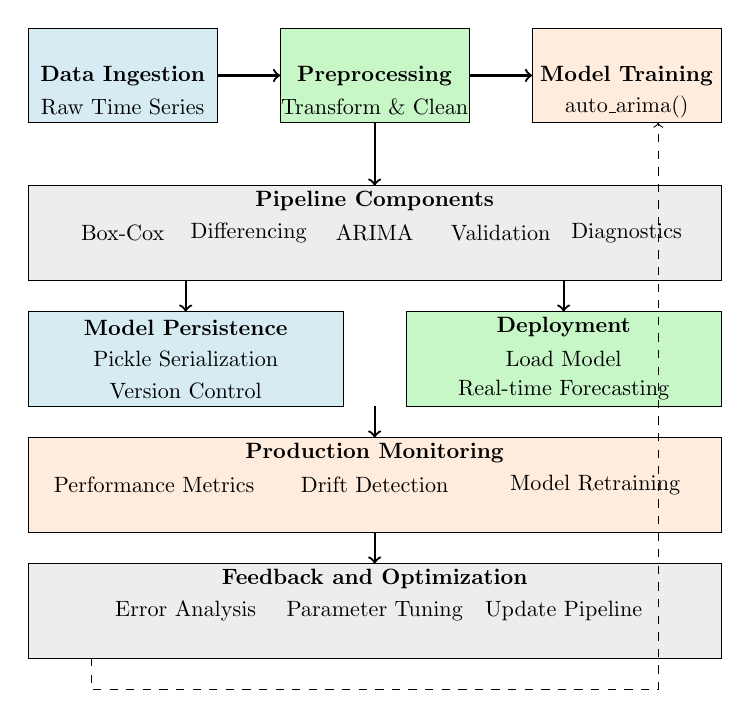
\begin{tikzpicture}[scale=0.8, every node/.style={scale=0.8}]

% Define colors
\definecolor{lightblue}{RGB}{173,216,230}
\definecolor{lightgreen}{RGB}{144,238,144}
\definecolor{lightorange}{RGB}{255,218,185}
\definecolor{lightgray}{RGB}{220,220,220}

% Data Ingestion
\draw[fill=lightblue!50] (0,9) rectangle (3,10.5);
\node at (1.5,9.75) {\textbf{Data Ingestion}};
\node at (1.5,9.25) {Raw Time Series};

% Preprocessing Pipeline
\draw[fill=lightgreen!50] (4,9) rectangle (7,10.5);
\node at (5.5,9.75) {\textbf{Preprocessing}};
\node at (5.5,9.25) {Transform \& Clean};

% Model Training
\draw[fill=lightorange!50] (8,9) rectangle (11,10.5);
\node at (9.5,9.75) {\textbf{Model Training}};
\node at (9.5,9.25) {auto\_arima()};

% Pipeline Components
\draw[fill=lightgray!50] (0,6.5) rectangle (11,8);
\node at (5.5,7.75) {\textbf{Pipeline Components}};
\node at (1.5,7.25) {Box-Cox};
\node at (3.5,7.25) {Differencing};
\node at (5.5,7.25) {ARIMA};
\node at (7.5,7.25) {Validation};
\node at (9.5,7.25) {Diagnostics};

% Model Serialization
\draw[fill=lightblue!50] (0,4.5) rectangle (5,6);
\node at (2.5,5.75) {\textbf{Model Persistence}};
\node at (2.5,5.25) {Pickle Serialization};
\node at (2.5,4.75) {Version Control};

% Deployment
\draw[fill=lightgreen!50] (6,4.5) rectangle (11,6);
\node at (8.5,5.75) {\textbf{Deployment}};
\node at (8.5,5.25) {Load Model};
\node at (8.5,4.75) {Real-time Forecasting};

% Monitoring
\draw[fill=lightorange!50] (0,2.5) rectangle (11,4);
\node at (5.5,3.75) {\textbf{Production Monitoring}};
\node at (2,3.25) {Performance Metrics};
\node at (5.5,3.25) {Drift Detection};
\node at (9,3.25) {Model Retraining};

% Feedback Loop
\draw[fill=lightgray!50] (0,0.5) rectangle (11,2);
\node at (5.5,1.75) {\textbf{Feedback and Optimization}};
\node at (2.5,1.25) {Error Analysis};
\node at (5.5,1.25) {Parameter Tuning};
\node at (8.5,1.25) {Update Pipeline};

% Arrows showing flow
\draw[->, thick] (3,9.75) -- (4,9.75);
\draw[->, thick] (7,9.75) -- (8,9.75);
\draw[->, thick] (5.5,9) -- (5.5,8);
\draw[->, thick] (2.5,6.5) -- (2.5,6);
\draw[->, thick] (8.5,6.5) -- (8.5,6);
\draw[->, thick] (5.5,4.5) -- (5.5,4);
\draw[->, thick] (5.5,2.5) -- (5.5,2);

% Feedback arrow
\draw[->, dashed] (1,0.5) -- (1,0) -- (10,0) -- (10,9);

\end{tikzpicture}
	\caption{Production Pipeline Architecture}
	\label{fig:pipelineDeployment}
\end{figure}

The production pipeline architecture illustrated in Figure \ref{fig:pipelineDeployment} demonstrates the end-to-end workflow from data ingestion to model deployment and monitoring.

\lstinputlisting[language=MyPython, caption={Pipeline Integration and Model Persistence}, label={lst:pipelineintegration},firstline=1,lastline=50]{../Code/pmdarima/PipelineIntegration.py}
\noindent\textit{The remaining code is omitted for brevity. The complete script can be found at \texttt{../Code/pmdarima/PipelineIntegration.py}.}

\section{Example -- Advanced Model Diagnostics}
\label{sec:diagnostics_example}

Comprehensive model diagnostics are crucial for validating ARIMA models and ensuring forecast reliability. This example demonstrates advanced diagnostic techniques and model evaluation.

\lstinputlisting[language=MyPython, caption={Advanced Model Diagnostics}, label={lst:diagnostics},firstline=1,lastline=50]{../Code/pmdarima/ModelDiagnostics.py}
\noindent\textit{The remaining code is omitted for brevity. The complete script can be found at \texttt{../Code/pmdarima/ModelDiagnostics.py}.}

\section{Performance Optimization}
\label{sec:optimization}

Optimizing pmdarima models requires understanding parameter selection strategies, computational efficiency, and memory management. Proper optimization ensures robust performance with large datasets and complex seasonal patterns.

\subsection{Parameter Selection Strategies}
\label{subsec:parameter_strategies}

Efficient parameter selection through stepwise and grid search approaches:

\begin{lstlisting}[language=MyPython, caption={Optimization Strategies}, label={lst:optimization}]
	import pmdarima as pm
	
	# Stepwise search (faster, recommended for most cases)
	stepwise_model = pm.auto_arima(
	    y, stepwise=True, seasonal=True, m=12,
	    suppress_warnings=True, error_action='ignore'
	)
	
	# Grid search (exhaustive, more accurate)
	grid_model = pm.auto_arima(
	    y, stepwise=False, seasonal=True, m=12,
	    max_p=3, max_q=3, max_P=2, max_Q=2,
	    suppress_warnings=True
	)
	
	# Parallel processing for large datasets
	parallel_model = pm.auto_arima(
	    y, seasonal=True, m=12, n_jobs=-1,
	    suppress_warnings=True
	)
\end{lstlisting}

\subsection{Memory and Computational Efficiency}
\label{subsec:efficiency}

Managing computational resources for large-scale forecasting:

\begin{lstlisting}[language=MyPython, caption={Efficiency Optimization}, label={lst:efficiency}]
	# Reduce search space for faster fitting
	efficient_model = pm.auto_arima(
	    y, start_p=0, start_q=0, max_p=2, max_q=2,
	    seasonal=True, m=12, stepwise=True,
	    suppress_warnings=True, error_action='ignore',
	    out_of_sample_size=int(len(y) * 0.1)  # Use validation set
	)
	
	# Memory-efficient batch processing
	def batch_forecast(data, batch_size=1000):
	    forecasts = []
	    for i in range(0, len(data), batch_size):
	        batch = data[i:i+batch_size]
	        model = pm.auto_arima(batch, suppress_warnings=True)
	        forecasts.extend(model.predict(10))
	    return forecasts
\end{lstlisting}

\section{Error Handling and Best Practices}
\label{sec:best_practices}

Robust pmdarima applications must handle various error conditions including convergence failures, non-stationary data, and invalid parameter combinations. Implementing comprehensive error handling ensures reliable forecasting systems.

\subsection{Common Issues and Solutions}
\label{subsec:common_issues}

\begin{enumerate}
	\item \textbf{Convergence Failures}: Use stepwise search and appropriate start parameters
	\item \textbf{Non-stationary Data}: Apply differencing or transformations before modeling
	\item \textbf{Seasonal Detection}: Manually specify seasonal parameters when auto-detection fails
	\item \textbf{Memory Issues}: Use out-of-sample validation and reduce search space
\end{enumerate}

\subsection{Production Error Handling Patterns}
\label{subsec:error_patterns}

\lstinputlisting[language=MyPython, caption={Comprehensive Error Handling}, label={lst:errorhandling},firstline=1,lastline=50]{../Code/pmdarima/ErrorHandling.py}
\noindent\textit{The remaining code is omitted for brevity. The complete script can be found at \texttt{../Code/pmdarima/ErrorHandling.py}.}

\section{Further Reading}
\label{sec:further_reading}

To deepen understanding of pmdarima and time series forecasting, consider these resources:

\subsection{Official Documentation}
\begin{itemize}
	\item \textbf{Pmdarima Documentation}: \url{https://alkaline-ml.com/pmdarima/}
	\item \textbf{GitHub Repository}: Official source code and examples \cite{Pmdarima:2024}
	\item \textbf{User Guide}: \url{https://alkaline-ml.com/pmdarima/user_guide.html}
	\item \textbf{API Reference}: \url{https://alkaline-ml.com/pmdarima/modules/generated/}
\end{itemize}

\subsection{Research and Tutorials}
\begin{itemize}
	\item \href{https://otexts.com/fpp2/}{Forecasting: Principles and Practice} by Hyndman and Athanasopoulos
	\item \href{https://towardsdatascience.com/time-series-forecasting-with-arima-sarima-and-sarimax-ee61099e78f6}{ARIMA, SARIMA, and SARIMAX Tutorial} \cite{TowardsDataScience:2023}
	\item \href{https://alkaline-ml.com/pmdarima/tips_and_tricks.html}{Tips and Tricks for Using auto\_arima}
\end{itemize}

\section{Conclusion}
\label{sec:conclusion}

Pmdarima provides a powerful and accessible solution for automated time series forecasting with Python. From simple univariate forecasting to complex seasonal models with exogenous variables, pmdarima's intuitive API and robust automation make it an essential tool for data scientists and analysts. The examples and techniques presented in this chapter provide a foundation for building production-ready forecasting systems, while the architectural understanding enables optimization for specific use cases and performance requirements.\\

Future developments in pmdarima focus on enhanced seasonal pattern detection, improved computational efficiency for large datasets, and expanded integration with modern ML frameworks \cite{Smith:2023}. As time series forecasting continues to evolve with increasing data volumes and complexity, pmdarima remains at the forefront of democratizing advanced statistical modeling, empowering practitioners worldwide to extract meaningful insights from temporal data through automated, reliable forecasting solutions.